

\documentclass{article}
\usepackage{amsmath,amssymb}
\usepackage{tikz}
\usepackage{enumitem}
\usetikzlibrary{arrows,shapes,automata,petri,positioning,calc}
\tikzset{
    place/.style={
        rectangle,
        thick,
        draw=black,
        fill=gray!50,
        minimum size=6mm,
    },
    lts/.style={
        ellipse,
        draw=black,
        fill=yellow!20,
        minimum size=8mm,
    },
    nfa/.style={
        ellipse,
        draw=black,
        fill=blue!20,
        minimum size=8mm,
    },
    prod/.style={
        ellipse,
        draw=black,
        fill=green!20,
        minimum size=10mm,
    },
    trace/.style={
        draw,
        -,>=stealth',
        semithick, 
    },
    trace-point/.style={
        circle,
        draw=black,
        fill=black,
        minimum size=3pt
    },
    every edge/.style={
        draw,
        ->,>=stealth',
        auto,
        semithick
    },
    initial text = {},
    node distance=2.5cm,
    double distance=2pt,
}

\begin{document}

\begin{enumerate}
    \item See Figure~\ref{fig:1} for labelled transition system
        \begin{figure}[htpb]
            \centering
                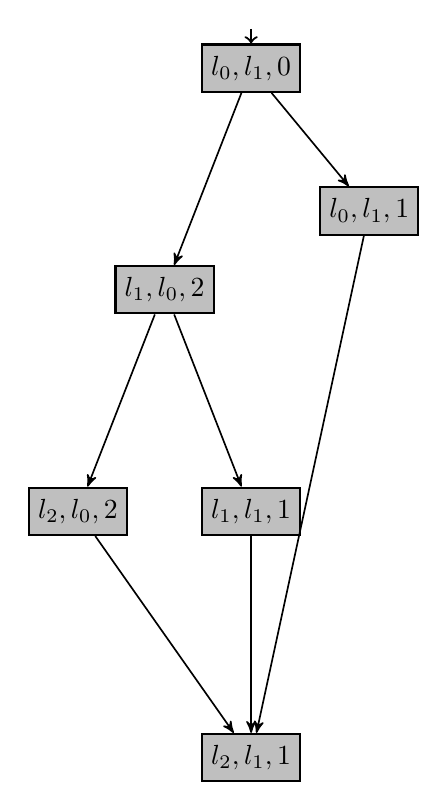
\begin{tikzpicture}

                    % Nodes and position definitions
                    \node [place] (N1) {$l_0,l_1,0$};
                    \coordinate[node distance=1.1cm,left of=N1] (left-N1);
                    \coordinate[node distance=1.5cm,right of=N1] (right-N1);
                    \coordinate[node distance=0.5cm,above of=N1] (above-N1);

                    \node [place] (S2) [below=of left-N1] {$l_1,l_0,2$};
                    \coordinate[node distance=1.1cm,left of=S2] (left-S2);
                    \coordinate[node distance=1.1cm,right of=S2] (right-S2);

                    \node [place] (S3) [node distance=1.5cm,below =of right-N1] {$l_0,l_1,1$};    
                    \coordinate[node distance=1.1cm,left of=S3] (left-S3);
                    \coordinate[node distance=1.1cm,right of=S3] (right-S3);

                    \node [place] (S4) [below=of left-S2] {$l_2,l_0,2$};
                    \coordinate[node distance=1.1cm,left of=S4] (left-S4);
                    \coordinate[node distance=1.1cm,right of=S4] (right-S4);

                    \node [place] (S5) [below=of right-S2] {$l_1,l_1,1$};
                    \coordinate[node distance=1.1cm,left of=S5] (left-S5);
                    \coordinate[node distance=1.1cm,right of=S5] (right-S5);

                    \node [place] (S6) [below=of S5]  {$l_2,l_1,1$};

                    % Vertex definitions
                    \draw[->, thick] (above-N1) -- (N1);
                    \path[->] (N1) edge node {} (S2);
                    \path[->] (N1) edge node {} (S3);
                    \path[->] (S2) edge node {} (S4);
                    \path[->] (S2) edge node {} (S5);
                    \path[->] (S4) edge node {} (S6);
                    \path[->] (S5) edge node {} (S6);
                    \path[->] (S3) edge node {} (S6);
                \end{tikzpicture}
            \caption{Question 1 Transition System}%
            \label{fig:1}
        \end{figure}

    \item 
        \begin{enumerate}[label=(\alph*)]
            \item whenever $a$ is true, $b$ is also true.
                \begin{equation}
                    \Box(a \rightarrow b)
                \end{equation}
                %This is an example of a safety property. This is the case as given a finite prefix $\sigma'$ including a state satisfying $a \wedge \neg b$, no infinite path can extend $\sigma'$ such that this property is satisfied.
                This is an example of a invariant. This is the case as it must always be true and it can be checked separately in each state.
                \begin{figure}[htpb]
                    \centering
                    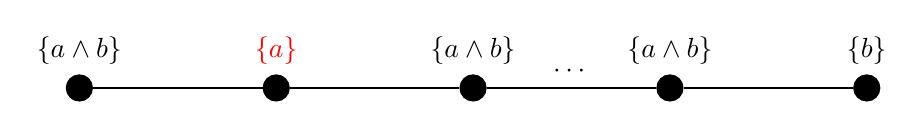
\begin{tikzpicture}
                        \node [trace-point, label=above:$\{a\wedge b\}$] (P1) {};
                        \node [trace-point,right of=P1,label=above:\color{red}$\{a\}$] (P2) {};
                        \node [trace-point,right of=P2,label=above:$\{a\wedge b\}$] (P3) {};
                        \node [trace-point,right of=P3,label=above:$\{a\wedge b\}$] at (5,0) (P4) {};
                        \node [trace-point,right of=P4,label=above:$\{b\}$] (P5) {};
                        \draw (P1) edge[-] node {} (P2);
                        \draw (P2) edge[-] node {} (P3);
                        \draw (P3) edge[-] node {$\cdots$} (P4);
                        \draw (P4) edge[-] node {} (P5);
                    \end{tikzpicture}
                    \caption{2 a, counterexample trace}%
                    \label{fig:2a}
                \end{figure}
            \item $a$ is eventually true
                \begin{equation}
                    \Diamond a
                \end{equation}
                This is an example of a liveness property as any finite word can be extended to satisfy this property. Any trace where $a$ never appears can be extended with a single case where $a$ is true \& it will now satisfy the property.
                \begin{figure}[htpb]
                    \centering
                    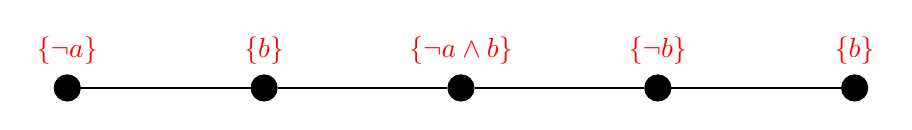
\begin{tikzpicture}
                        \node [trace-point, label=above:\color{red}$\{\neg a\}$] (P1) {};
                        \node [trace-point,right of=P1,label=above:\color{red}$\{b\}$] (P2) {};
                        \node [trace-point,right of=P2,label=above:\color{red}$\{\neg a\wedge b\}$] (P3) {};
                        \node [trace-point,right of=P3,label=above:\color{red}$\{\neg b\}$] at (5,0) (P4) {};
                        \node [trace-point,right of=P4,label=above:\color{red}$\{b\}$] (P5) {};
                        \draw (P1) edge[-] node {} (P2);
                        \draw (P2) edge[-] node {} (P3);
                        \draw (P3) edge[-] node {} (P4);
                        \draw (P4) edge[-] node {} (P5);
                    \end{tikzpicture}
                    \caption{2 b, counterexample trace}%
                    \label{fig:2b}
                \end{figure}
            \item $a$ eventually comes true but is then subsequently false again.
                \begin{equation}
                    \Diamond a \rightarrow (a \wedge \bigcirc \neg a)
                \end{equation}
                This is a safety property as any violation produces a trace that cannot be extended into a satisfactory trace.
                \begin{figure}[htpb]
                    \centering
                    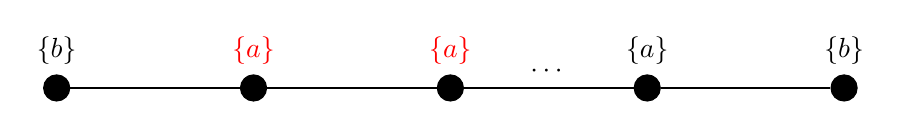
\begin{tikzpicture}
                        \node [trace-point, label=above:$\{ b\}$] (P1) {};
                        \node [trace-point,right of=P1,label=above:\color{red}$\{a\}$] (P2) {};
                        \node [trace-point,right of=P2,label=above:\color{red}$\{a\}$] (P3) {};
                        \node [trace-point,right of=P3,label=above:$\{a\}$] at (5,0) (P4) {};
                        \node [trace-point,right of=P4,label=above:$\{b\}$] (P5) {};
                        \draw (P1) edge[-] node {} (P2);
                        \draw (P2) edge[-] node {} (P3);
                        \draw (P3) edge[-] node {$\cdots$} (P4);
                        \draw (P4) edge[-] node {} (P5);
                    \end{tikzpicture}
                    \caption{2 c, counterexample trace}%
                    \label{fig:2c}
                \end{figure}
            \item $a$ and $b$ are both true infinitely often, but never simultaneously.
                \begin{equation}
                    \Box \Diamond a \wedge \Box\Diamond b \wedge \Box\neg(a \wedge b)
                \end{equation}
                This is a safety property as if the final clause of the property ($\Box \neg(a\wedge b)$) is unsatisfied in one state, the entire trace is invalidated and cannot be extended into a valid trace.
                \begin{figure}[htpb]
                    \centering
                    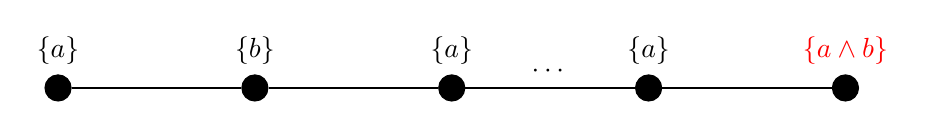
\begin{tikzpicture}
                        \node [trace-point, label=above:$\{ a\}$] (P1) {};
                        \node [trace-point,right of=P1,label=above:$\{b\}$] (P2) {};
                        \node [trace-point,right of=P2,label=above:$\{a\}$] (P3) {};
                        \node [trace-point,right of=P3,label=above:$\{a\}$] at (5,0) (P4) {};
                        \node [trace-point,right of=P4,label=above:\color{red}$\{a\wedge b\}$] (P5) {};
                        \draw (P1) edge[-] node {} (P2);
                        \draw (P2) edge[-] node {} (P3);
                        \draw (P3) edge[-] node {$\cdots$} (P4);
                        \draw (P4) edge[-] node {} (P5);
                    \end{tikzpicture}
                    \caption{2 d, counterexample trace}%
                    \label{fig:2d}
                \end{figure}
            \item the first occurrence (if any) of $a$ is immediately followed by $b$
                \begin{equation}
                    a \vee b \cup a \rightarrow \bigcirc b
                \end{equation}
                This is an example of a safety property as any finite word $\sigma'$ that does not satisfy the property cannot be extended by any infinite word such that it now satisfies the property.
                \begin{figure}[htpb]
                    \centering
                    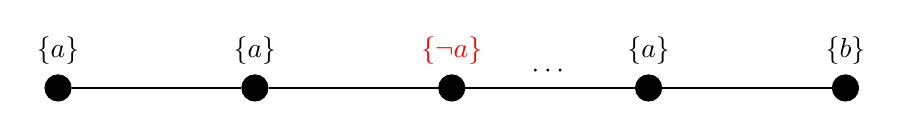
\begin{tikzpicture}
                        \node [trace-point, label=above:$\{ a\}$] (P1) {};
                        \node [trace-point,right of=P1,label=above:$\{a\}$] (P2) {};
                        \node [trace-point,right of=P2,label=above:\color{red}$\{\neg a\}$] (P3) {};
                        \node [trace-point,right of=P3,label=above:$\{a\}$] at (5,0) (P4) {};
                        \node [trace-point,right of=P4,label=above:$\{b\}$] (P5) {};
                        \draw (P1) edge[-] node {} (P2);
                        \draw (P2) edge[-] node {} (P3);
                        \draw (P3) edge[-] node {$\cdots$} (P4);
                        \draw (P4) edge[-] node {} (P5);
                    \end{tikzpicture}
                    \caption{2 e, counterexample trace}%
                    \label{fig:2e}
                \end{figure}
        \end{enumerate}

    \item We first negate the safety property, $\Psi$, giving us $\neg\Psi$ in Equation~\ref{eq:negpsi}. Constructing a NFA of this property gives us $\mathcal{A}_{\neg\Psi}$ shown in Figure~\ref{fig:3-nfa}. The product of $M$ and $\mathcal{A}_{\neg\Psi}$, $M \otimes \mathcal{A}_{\neg\Psi}$ is shown in Figure~\ref{fig:3-ans}. This graph has an accept state so therefore this property does not hold for the LTS $M$.
        \begin{equation}
            \Psi = \Box\left(a \rightarrow \bigcirc\Box b\right)
        \end{equation}
        \begin{figure}[htpb]
            \centering
            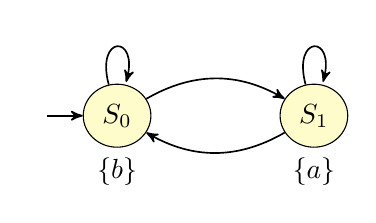
\begin{tikzpicture}
                \node [lts,initial, label=below:$\{b\}$] (S0) {$S_0$};

                \node [lts, right of=S0, label=below:$\{a\}$] (S1) {$S_1$};

                \draw (S0) edge[loop above] node {} (S0);
                \draw (S1) edge[loop above] node {} (S1);
                \draw (S0) edge[bend left] node {} (S1);
                \draw (S1) edge[bend left] node {} (S0);



            \end{tikzpicture}
            \caption{LTS-$M$}%
            \label{fig:3-M}
        \end{figure}
        \begin{multline}\label{eq:negpsi}
            \begin{aligned}
                \neg\Psi &= \neg \Box(a \rightarrow \bigcirc\Box b) \\
                   &\equiv \Diamond\neg(a \rightarrow \bigcirc\Box b) \\
                   &\equiv \Diamond\neg(\neg a \vee \bigcirc\Box b) \\
                   &\equiv \Diamond(a \wedge \neg\bigcirc\Box b) \\
                   &\equiv \Diamond(a \wedge \bigcirc\neg\Box b) \\
                   &\equiv \Diamond(a \wedge \bigcirc\Diamond\neg b) 
            \end{aligned}
        \end{multline}
        \begin{figure}[htpb]
            \centering
            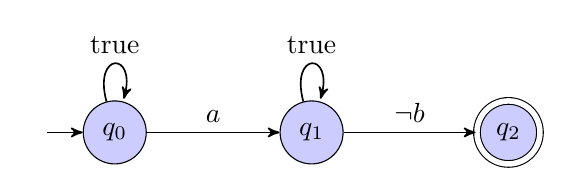
\begin{tikzpicture}
                \node [nfa, initial] (Q0) {$q_0$}; 
                \node [nfa, right of=Q0] (Q1) {$q_1$};
                \node [nfa,accepting, right of=Q1] (Q2) {$q_2$};

                \draw (Q0) edge[loop above] node {true} (Q0);
                \draw (Q0) edge node {$a$} (Q1);
                \draw (Q1) edge[loop above] node {true} (Q1);
                \draw (Q1) edge node {$\neg b$} (Q2);
            \end{tikzpicture}
            \caption{NFA-$\mathcal{A}_{\neg\Psi}$}%
            \label{fig:3-nfa}
        \end{figure}        
        \begin{figure}[htpb]
            \centering
            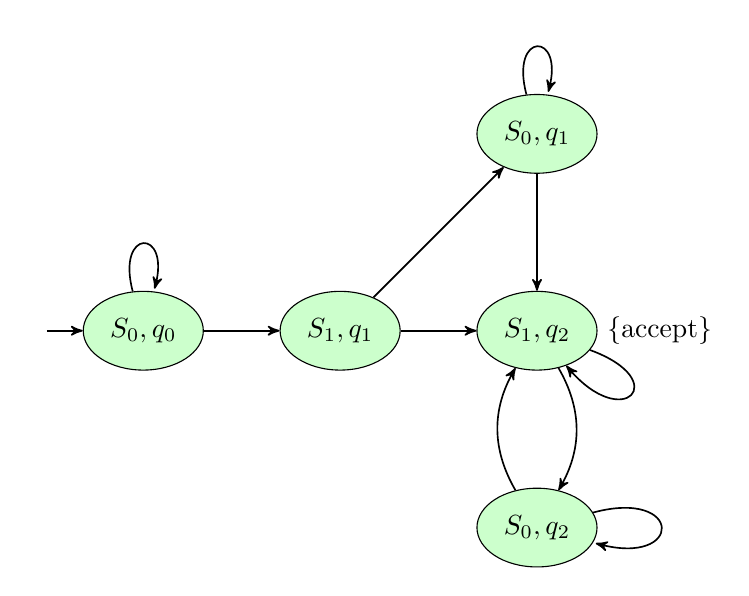
\begin{tikzpicture}
                \node [prod, initial] (S0Q0) {$S_0, q_0$};
                \node [prod, right of=S0Q0] (S1Q1) {$S_1, q_1$};
                \node [prod, right of=S1Q1, label=right:$\{$accept$\}$] (S1Q2) {$S_1,q_2$};
                \node [prod, above of=S1Q2] (S0Q1) {$S_0,q_1$};
                \node [prod, below of=S1Q2] (S0Q2) {$S_0,q_2$};

                \draw (S0Q0) edge[loop above] node {} (S0Q0);
                \draw (S0Q0) edge node {} (S1Q1);
                \draw (S1Q1) edge node {} (S0Q1);
                \draw (S1Q1) edge node {} (S1Q2);

                \draw (S0Q1) edge[loop above] node {} (S0Q1);
                \draw (S0Q1) edge node {} (S1Q2);

                \draw (S1Q2) edge[out=340, in=310, looseness=8] node {} (S1Q2);
                \draw (S1Q2) edge[bend left] node {} (S0Q2);

                \draw (S0Q2) edge[loop right] node {} (S0Q2);
                \draw (S0Q2) edge[bend left] node {} (S1Q2);

                
            \end{tikzpicture}
            \caption{$M \otimes \mathcal{A}_{\neg\Psi}$}%
            \label{fig:3-ans}
        \end{figure}
\end{enumerate}

\end{document}
